%
% $RCSfile: human_thinking.tex,v $
%
% Copyright (c) 2001-2004. Christian Heller. All rights reserved.
%
% No copying, altering, distribution or any other actions concerning this
% document, except after explicit permission by the author!
% At some later point in time, this document is planned to be put under
% the GNU FDL license. For now, _everything_ is _restricted_ by the author.
%
% http://www.cybop.net
% - Cybernetics Oriented Programming -
%
% http://www.resmedicinae.org
% - Information in Medicine -
%
% @author Christian Heller <christian.heller@tuxtax.de>
%

\section{Human Thinking}
\label{human_thinking_heading}

Criticising \emph{State-of-the-Art} concepts is one part of science; offering
improved solutions is its complementary.
Researchers quite often follow the approach of first looking into what nature
offers and then trying to engineer a similar solution. All kinds of tools and
machines were created this way, even (and most obviously, with respect to the
human body and mind) robots and computers. Some scientists take the principles
of human awareness as physical model to explain the universe \cite{ripota}.
Some business people and consultants see analogies between processes in the
human brain and organisational structures of a company \cite{schoenhofer}.
Researchers in human sciences systematise international public law by sharing it
into the three parts society, cooperation and conflicts which are chosen in analogy
to biology, that is anatomy, physiology and pathology of international relations
\cite{bierzanek}. Considering all that, one question is at hand:

\begin{center}
    \textbf{Why not apply a similar approach to\\
    software engineering?}
\end{center}

The science of \emph{Cybernetics} and its specialization \emph{Bionics} recommend
to \emph{compare} communication and control processes in biological versus
artificial systems as well as to \emph{apply} biological principles to the
study and design of engineering systems. If computers are built after the model of
the human being (information input, memorizing, processing and output), why not
structure the software that actually runs those computers after similar models?
It seems logical and clear, yet the reality looks different. This section will
therefore consider how \emph{Human Thinking} works and how it creates abstractions
(figure \ref{human_thinking_figure}).

\begin{figure}[ht]
    \begin{center}
        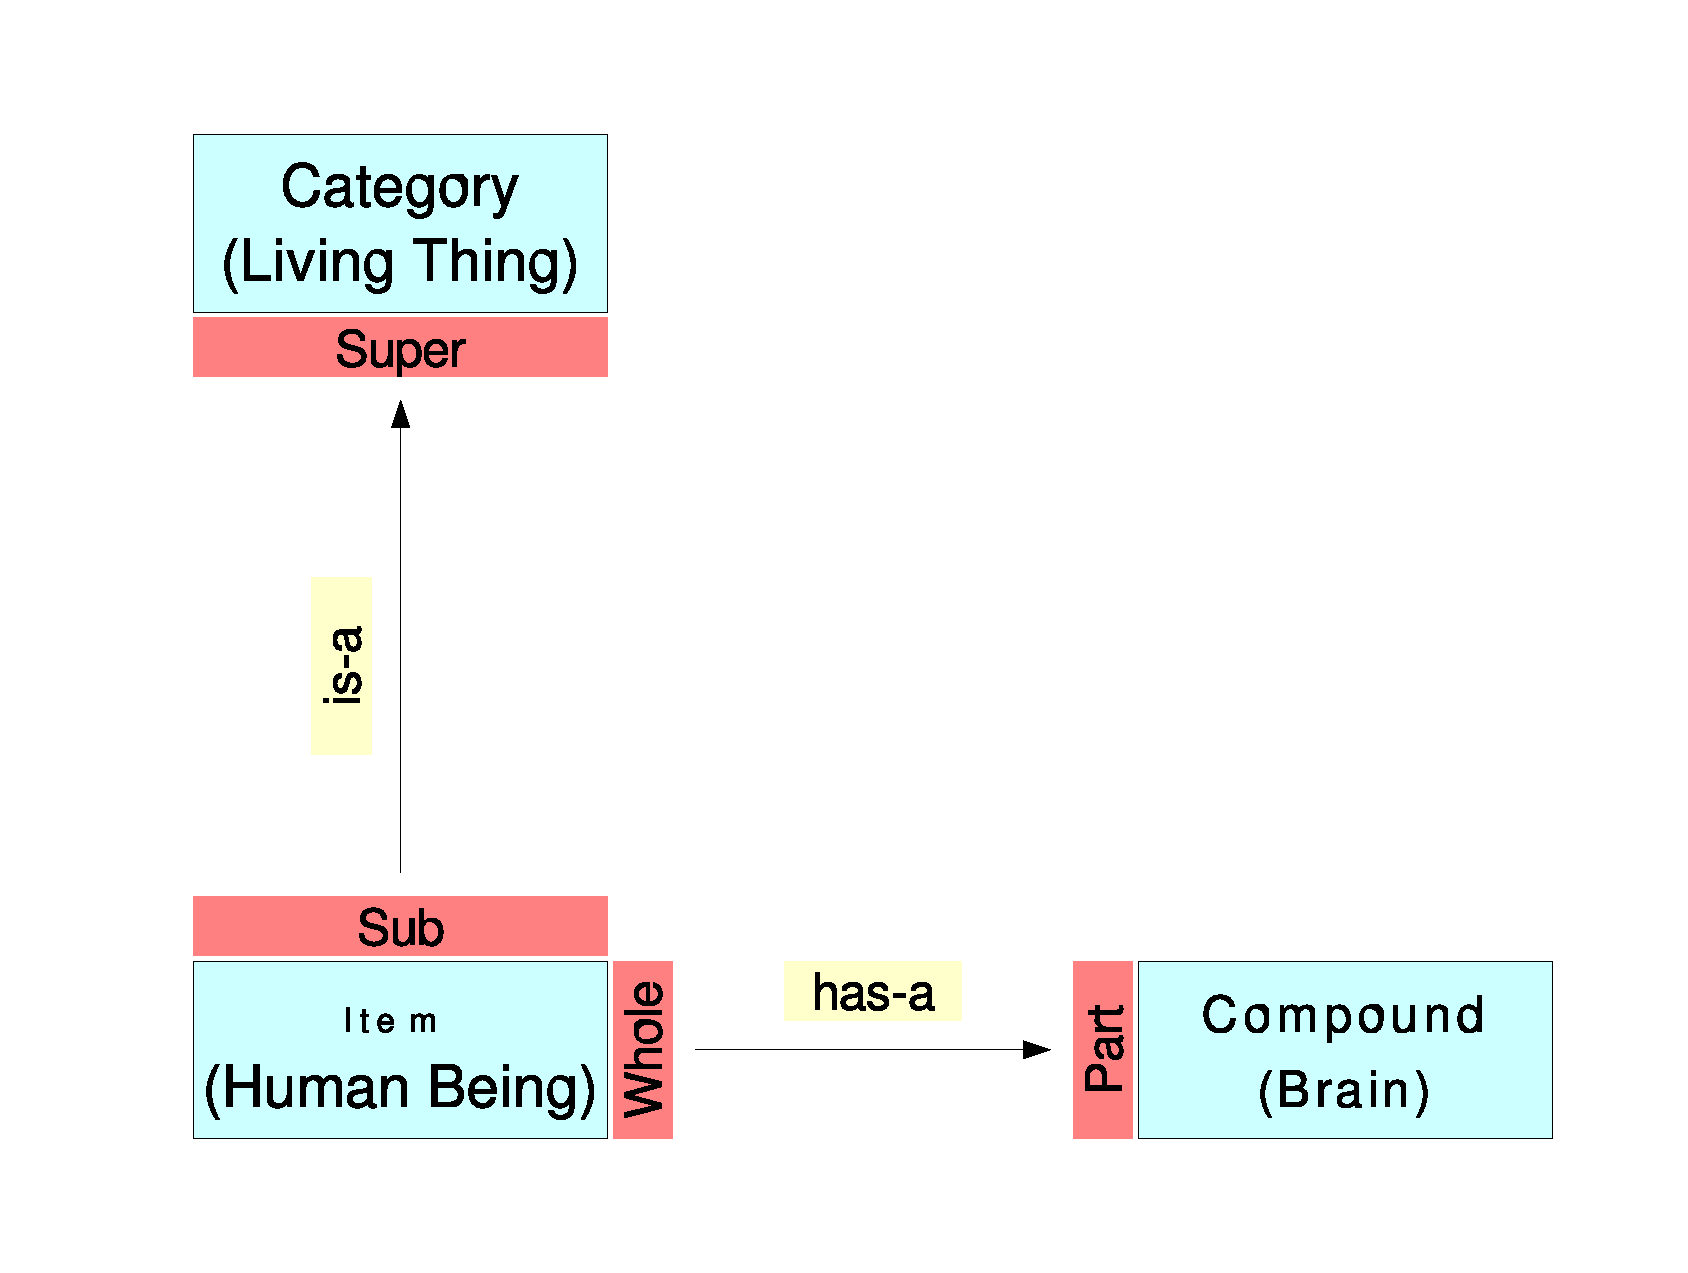
\includegraphics[scale=0.3]{vector/human_thinking.eps}
        \caption{Human Thinking}
        \label{human_thinking_figure}
    \end{center}
\end{figure}

%
% $RCSfile: item.tex,v $
%
% Copyright (c) 2001-2004. Christian Heller. All rights reserved.
%
% No copying, altering, distribution or any other actions concerning this
% document, except after explicit permission by the author!
% At some later point in time, this document is planned to be put under
% the GNU FDL license. For now, _everything_ is _restricted_ by the author.
%
% http://www.cybop.net
% - Cybernetics Oriented Programming -
%
% http://www.resmedicinae.org
% - Information in Medicine -
%
% @author Christian Heller <christian.heller@tuxtax.de>
%

\subsection{Item}
\label{item_heading}

As first and most important abstraction, the human brain divides its real-world
environment into discrete \emph{Items}. Physicists call smaller items \emph{Particle}.
Plenty of other synonyms exist. Software developers often talk of \emph{Object}.
This document preferrably uses the more neutral name \emph{Item}, since models
are created not only of objects but also of \emph{Subjects}.

Behavioural psychologists talk of this ability as \emph{Discrimination}. It commonly
focuses on a specific real world phenomenon, leaving out parameters which are not
interesting in the given context. This is necessary because otherwise, a brain
would have to model and capture the whole universe (with every single particle
being duplicated), which is obviously impossible. As example, a \emph{Human Being}
as item is stated (in parentheses) in figure \ref{human_thinking_figure}.

Not only human beings, but also some higher animal species (like apes) are able
to \emph{discriminate} their environment and to form terms to name it.
Additionally, they have a primitive \emph{Self Concept}, that is a term for
their own personality. However, their cognitive abilities are limited in that
concepts are only available in the presence of the corresponding item. Jaeger
\cite{jaeger} calls that \emph{Online Thinking}; cognition scientists speak of
\emph{Terms of first Order} or \emph{Sensoric Type of Terms}.

Contrary to this, the more advanced \emph{Offline Thinking} allows humans to
think about items they currently cannot sense. Cognition scientists here speak of
\emph{Terms of second Order}. They became possible by \emph{associating} sensoric
signals with terms of a language. The resulting \emph{Net of Associations} brought
a number of advantages \cite{jaeger}:

\begin{itemize}
    \item{\emph{Decoupling} thinking from immediate motoric reaction}
    \item{\emph{Time Index} in scenes so that past memories can be\\
        recalled, the future be planned}
    \item{\emph{Dual Representation} of online and offline contents}
    \item{\emph{Self Awareness} thanks to online and offline thinking}
    \item{\emph{Associations} increasing the expressiveness of terms}
\end{itemize}

%
% $RCSfile: category.tex,v $
%
% Copyright (c) 2001-2004. Christian Heller. All rights reserved.
%
% No copying, altering, distribution or any other actions concerning this
% document, except after explicit permission by the author!
% At some later point in time, this document is planned to be put under
% the GNU FDL license. For now, _everything_ is _restricted_ by the author.
%
% http://www.cybop.net
% - Cybernetics Oriented Programming -
%
% http://www.resmedicinae.org
% - Information in Medicine -
%
% @author Christian Heller <christian.heller@tuxtax.de>
%

\subsection{Category}
\label{category_heading}

Offline thinking (in terms of second order) enables humans not only to
discriminate items but also to \emph{categorize} them into superior groups.
Since it is impossible to exactly model the real world in complete, compromises
have to be made: People do not model every single item in their minds but rather
group them into \emph{Types} (\emph{Classes}) of common characteristics.

This kind of classification stems from the earliest days of ancient science.
\emph{Plato}'s pupil \emph{Aristotle} (being the teacher of \emph{Alexander the
Great}) was the first philosopher who logically captured and organized the world.
It was him who sorted items into clear groups which he called \emph{Categories}.
And it was him who first distinguished between \emph{enlivened} and
\emph{unenlivened} nature; who parted living forms into \emph{Plants},
\emph{Animals} and \emph{Humans}. The science of biology calls this classification
a \emph{Systematics}.

\emph{Categorization} (classification) can be seen from two sides, depending on
what direction of that relationship one wants to emphasize. Taking Aristotle's
examples, \emph{Living Thing} would be a \emph{Generalization} of \emph{Plants},
\emph{Animals} and \emph{Humans}. \emph{Human Being} would be a \emph{Specialization}
of \emph{Living Thing}.

Software developers call categorization an \emph{is-a} relationship and talk of
\emph{Super} and \emph{Sub} categories (sometimes also \emph{Parent} and
\emph{Child} categories). Section \ref{property_bundling_heading} mentioned that
object oriented programming uses categorization to let a sub class inherit
attributes and methods from its super class.

%
% $RCSfile: compound.tex,v $
%
% Copyright (C) 2002-2008. Christian Heller.
%
% Permission is granted to copy, distribute and/or modify this document
% under the terms of the GNU Free Documentation License, Version 1.1 or
% any later version published by the Free Software Foundation; with no
% Invariant Sections, with no Front-Cover Texts and with no Back-Cover
% Texts. A copy of the license is included in the section entitled
% "GNU Free Documentation License".
%
% http://www.cybop.net
% - Cybernetics Oriented Programming -
%
% http://www.resmedicinae.org
% - Information in Medicine -
%
% Version: $Revision: 1.1 $ $Date: 2008-08-19 20:41:06 $ $Author: christian $
% Authors: Christian Heller <christian.heller@tuxtax.de>
%

\subsubsection{Compound}
\label{compound_heading}
\index{Compound}
\index{Composition}
\index{Tree}
\index{Hierarchy}
\index{Artificial Intelligence}
\index{AI}
\index{Concept}
\index{Schema}
\index{Monades Theory}
\index{Parent Item}
\index{Child Item}
\index{Whole}
\index{Part}
\index{Container}
\index{Element}
\index{Genealogy}
\index{Unidirectional Relation}
\index{Hierarchical State}
\index{Hierarchical Procedure}
\index{Microcosm}
\index{Macrocosm}
\index{Particle}

\emph{Composition} is the third kind of abstraction that humans use to
understand their environment. It is an important instrument for the human mind
to associate information, that is to acquire, store and recall \emph{Knowledge}.
Every item can be recognised as a \emph{Compound} of smaller items and can
therefore also be called \emph{Tree} or \emph{Hierarchy}. The subject of
\emph{Artificial Intelligence} (AI) talks of \emph{Concept} or \emph{Schema}
\cite{sowa}.

The great philosopher and mathematician Gottfried Wilhelm Leibnitz (1646-1716)
made extensive use of the principle of hierarchy. His entire theory of
\emph{Monades} \cite{leibnitz} is based on it.

In software design, the terms \emph{Parent} and \emph{Child} are often used to
describe both, the items in a composition relation and the items in a
categorisation (inheritance) relationship. To avoid misunderstandings, this
work sticks to the terms \emph{Super} and \emph{Sub} for categorisation and to
the terms \emph{Whole} and \emph{Part} for composition. Yet other terms to
describe items of a composition would be \emph{Container} and \emph{Element}.

One obvious analogy comes from \emph{Genealogy} where parents have children who
become parents of their own children and so forth. Displaying these relations
between family members in a graph, leads to a tree which may represent both,
a category tree (for property inheritance) as well as a composition tree (for
children ownership).

Taking the example of a \emph{Human Being}, one could say that it is composed
of organs such as \emph{Eye}, \emph{Ear}, \emph{Heart}, \emph{Brain},
\emph{Arm} and further, also smaller parts. John F. Sowa \cite[p. 109]{sowa}
writes on this:

\begin{quote}
    From different viewpoints, the human body can be considered an aggregate of
    organs, an aggregate of cells, or an aggregate of molecules. Each viewpoint
    affects the terminology used to talk about the body, but not the body itself.
\end{quote}

That is, one and the same real world object may be represented in many
different ways. It is important to note the \emph{unidirectional} kind of
relations: A human being is composed of organs but an organ is never composed
of a human being! Another example is that of a \emph{Book}: physically, it may
be composed of a \emph{Paperback Cover} and \emph{Paper Pages}; logically,
however, it is usually separated into \emph{Part}, \emph{Chapter},
\emph{Section}, \emph{Paragraph}, \emph{Sentence}, \emph{Word} and
\emph{Character}. Obviously, knowledge representation always depends on what
one wants to express in which context. Philippe Ameline who works in the
\emph{Nautilus-Odyssee} project \cite{nautilus}, writes in \cite{openhealth}:

\begin{quote}
    Lets take a comparison with \emph{Geography}: you can build an ontology
    (which consists of compound structures) in order to describe natural
    objects (mountains, rivers, \ldots). But if you build artificial frontiers
    and call them \emph{Countries}, you cannot semantically include these
    concepts inside the geographical domain. -- That is the very reason why
    human beings, very frustrated, had to invent the political domain ;-)
    \ldots\ I think that there (are similar differences) in medicine (as in)
    the geographical domain.
\end{quote}

Not only \emph{States} may be represented as compound; \emph{Procedures} may be
hierarchical as well. The process \emph{Take Book from Library}, for example,
may have the following structure:

\begin{itemize}
    \item[-] Check Catalogue
    \begin{itemize}
        \item[-] Investigate suitable Books
        \item[-] Note Registration Number
    \end{itemize}
    \item[-] Obtain Book
    \begin{itemize}
        \item[-] Look for Shelf
        \item[-] Take off Book
    \end{itemize}
    \item[-] Borrow Book
\end{itemize}

Returning to human thinking, one realises that in the end, everything in
universe can be put into variable hierarchical models, that is consists of
smaller items and belongs to a bigger item. From the physical point of view,
nobody knows where this hierarchy really stops, towards \emph{Microcosm} as
well as towards \emph{Macrocosm}. There is no \emph{absolute}, \emph{basic}
item. A \emph{Particle} as concept exists only in the human mind, placed
somewhere between micro- and macrocosm, with hypothetic borders.

%
% $RCSfile: model.tex,v $
%
% Copyright (c) 2001-2004. Christian Heller. All rights reserved.
%
% No copying, altering, distribution or any other actions concerning this
% document, except after explicit permission by the author!
% At some later point in time, this document is planned to be put under
% the GNU FDL license. For now, _everything_ is _restricted_ by the author.
%
% http://www.cybop.net
% - Cybernetics Oriented Programming -
%
% http://www.resmedicinae.org
% - Information in Medicine -
%
% @author Christian Heller <christian.heller@tuxtax.de>
%

\subsection{Model}
\label{model_heading}

A theoretical \emph{Model} is an abstract clip of the real world, and exists in
the human mind. Another common word for \emph{Model} is \emph{Concept}.
It is the subsumption of \emph{Item}, \emph{Category} and \emph{Compound},
resulting from the three activities of abstraction: \emph{Discrimination},
\emph{Categorization} and \emph{Composition}. As such, each model knows about
its super model and the parts it consists of (figure \ref{abstract_model_figure}).
Software developers would call the illustration of these relations a \emph{Schema}
or \emph{Meta Model}.

\begin{figure}[ht]
    \begin{center}
        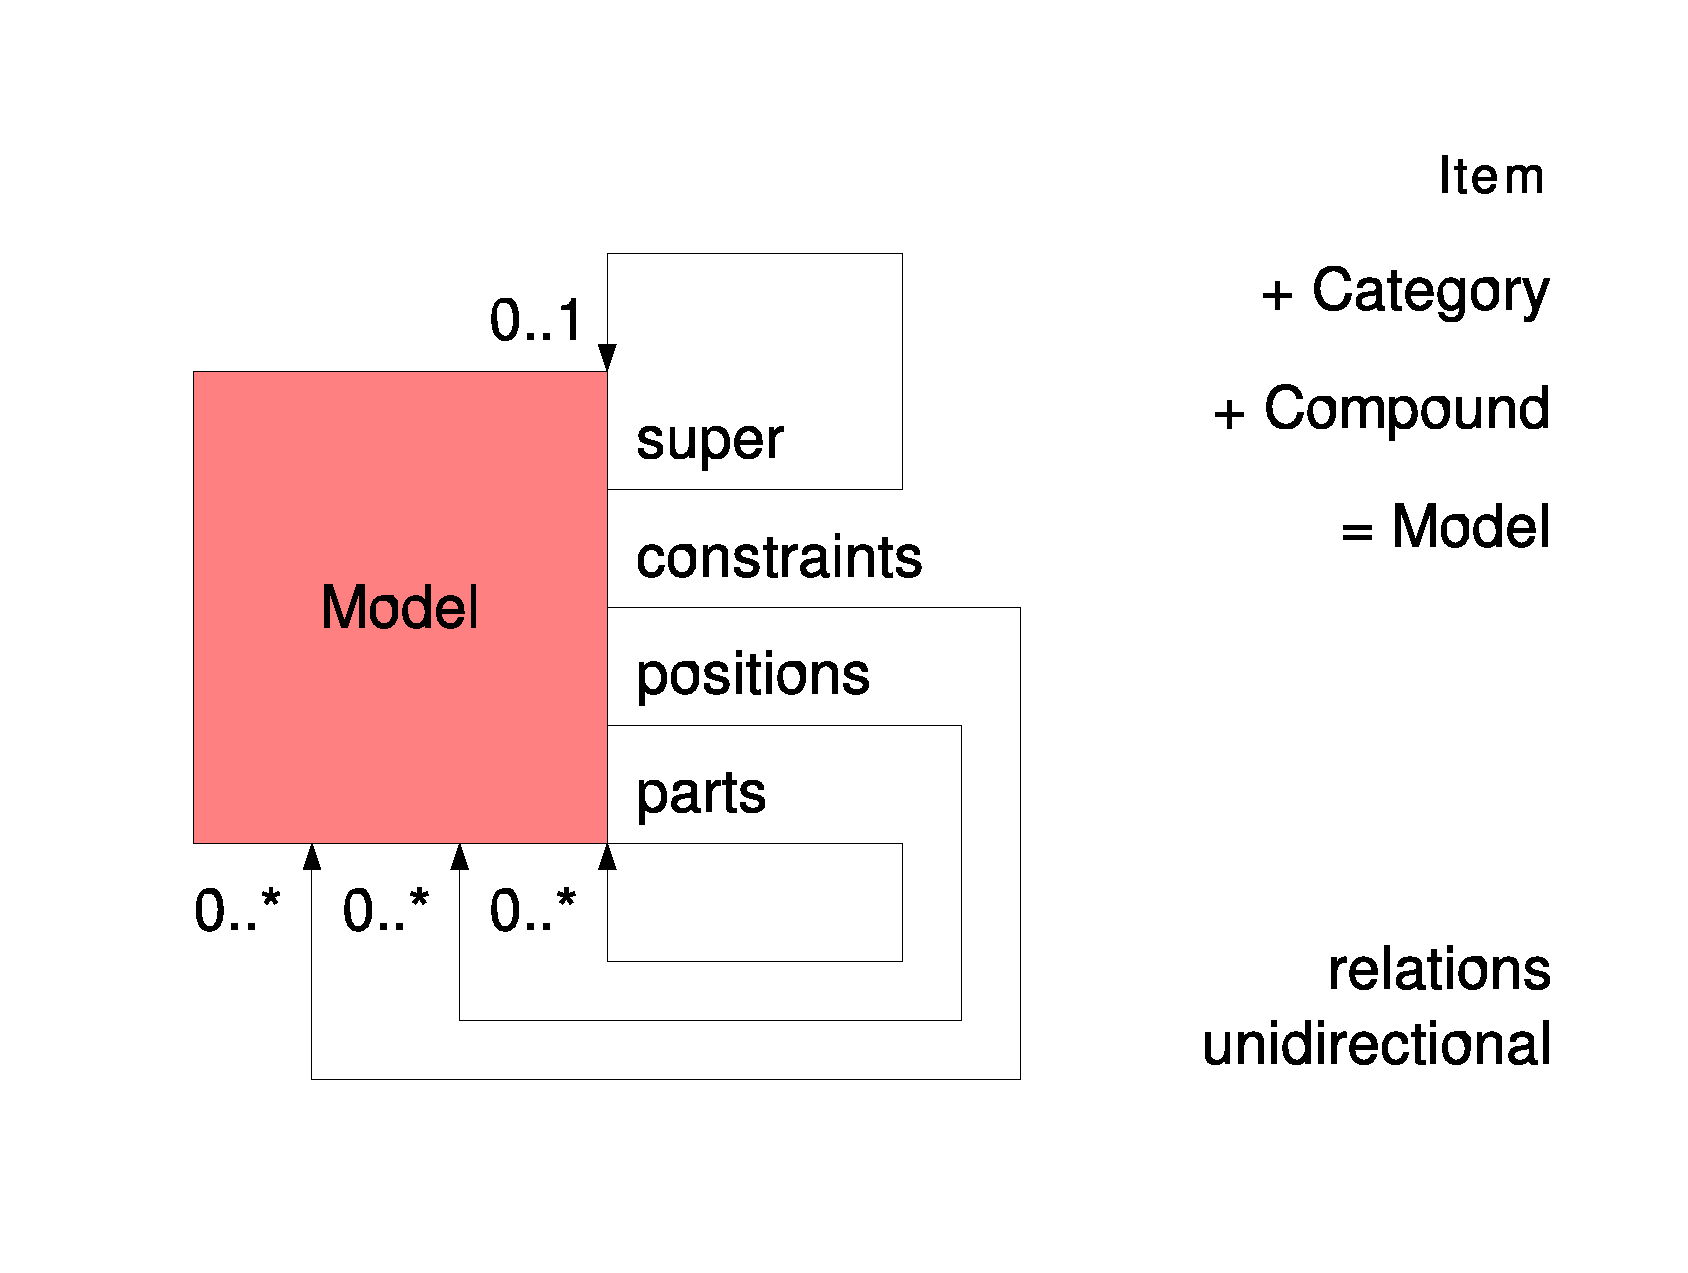
\includegraphics[scale=0.3]{vector/abstract_model.eps}
        \caption{Model as subsumption of Item, Category, Compound}
        \label{abstract_model_figure}
    \end{center}
\end{figure}

%
% $RCSfile: interaction.tex,v $
%
% Copyright (c) 2001-2004. Christian Heller. All rights reserved.
%
% No copying, altering, distribution or any other actions concerning this
% document, except after explicit permission by the author!
% At some later point in time, this document is planned to be put under
% the GNU FDL license. For now, _everything_ is _restricted_ by the author.
%
% http://www.cybop.net
% - Cybernetics Oriented Programming -
%
% http://www.resmedicinae.org
% - Information in Medicine -
%
% @author Christian Heller <christian.heller@tuxtax.de>
%

\subsection{Interaction}
\label{interaction_heading}

As explained in previous sections, every abstract model is a \emph{Compound} of
smaller \emph{Parts}. What does this relation imply? What does a compound
\emph{know} about its parts? Knowledge \emph{about} something is often called
\emph{Meta Information}.

The most obvious way to uniquely identify parts is to give them a \emph{Name}. The
concept of a human body, for example, has parts like \emph{Heart}, \emph{Left Arm}
or \emph{Skin}. Secondly, a compound needs to know about the \emph{Model} of each
part which may be a compound itself. But what about other knowledge like
the order or position of parts within their compound?

To find an answer, the science of \emph{Psychology} needs to be called in. It
distinguishes between various aspects of a (visual) impression of the human mind,
as there are \emph{Shape}, \emph{Depth}, \emph{Color} or \emph{Movement}
\cite{stoerig}. Looking closer at these, one realizes that they are representations
of the classical physical dimensions that humans use to describe the world:

\begin{itemize}
    \item{\emph{Movement}: changing the state of something over \emph{Time}}
    \item{\emph{Shape}: how items would appear in a two-dimensional world, as
        known from \emph{Geometry}}
    \item{\emph{Depth} (stereo vision): adding a third dimension to shapes, so
        that these become three-dimensional and form a \emph{Space}}
    \item{\emph{Color}: not being considered a dimension, telling about how items
        reflect \emph{Light}}
    \item{\emph{Mass}: another physical value describing the world which is not
        considered to be a dimension}
\end{itemize}

If, according to modern physics, not all of the impressions listed above are
dimensions, what is common to them? -- All can be used to express a special aspect
of a composition relation which this paper calls \emph{Composition Interaction}.

To the concept of an \emph{Atom} belong a \emph{Core} and \emph{Electrons}. The
atom provides the \emph{Space} that the core and electrons can fill with their
extension. For core and electrons, the atom represents the small universe they live
in. Moreover, the atom \emph{knows} about the \emph{Position} (\emph{Trajectory})
of each electron. Thus, one can say that the atom as a \emph{Whole} interacts with
its \emph{Parts} by means of space. Electrons, on the other hand, know nothing
about their own position within the atom; they do not know about the existence of
the atom at all. But having a size, they indirectly exert influence on the whole
atom by contributing to its overall extension in space.

A \emph{Solar System}, as concept, has very much in common with the atom. It has a
star, the \emph{Sun}, as its core and it has \emph{Planets} orbiting around that
star. Besides the composition interaction over space that also exists here, there
is another relation worth paying attention to: \emph{Mass}. Conceptually, the
solar system can be treated as a closed field of \emph{Mass}, the sun representing
the center of that mass, the planets additions. The solar system as a \emph{Whole}
knows about the masses of its \emph{Parts}, what can be considered a conceptual
interaction.

A third relation that humans use to place themselves and the environment into their
very own model of the universe is \emph{Time}. Any \emph{Process} can be split into
\emph{Sub Processes} and such represents a structure with \emph{hierarchical}
character. In most cases, the \emph{Order} in which sub processes are executed, is
very important. Without it, no meaningful \emph{Algorithm} could ever be created.
A process knows about the \emph{Occurrence} of its sub processes and this sequence
information is stored in units of time. Moreover, the \emph{Whole} process sets a
time frame that all \emph{Part} processes, in sum, cannot exceed. Their \emph{Duration}
is limited. Again, process and sub processes have some kind of composition relation;
in this case over time.

Conceptual interactions like \emph{Space}, \emph{Mass} or \emph{Time} are used by a
model to position parts within its area of validity. Yet this meta knowledge is not
enough. Frequently, parts have to be \emph{constrained} to maintain the validity of
the whole model. The concept of a \emph{Table} consists of a \emph{Top} and one to
four \emph{Legs}. The additional information herein is the \emph{Constraint} of the
number of legs to at least \emph{one} and at most \emph{four}.

Finally, what makes up the \emph{Character} of an item (in the understanding of the
human mind) is the \emph{Parts} it consists of, combined with \emph{Meta Information}
about these parts. Most properties of a molecule in \emph{Chemistry} are determined
by the number and arrangement of its atoms. \emph{Hydrogen} (H$_{2}$) becomes
\emph{Water} (H$_{2}$O) (with a totally different character) when one \emph{Oxygen}
(O) atom is added per hydrogen molecule.

Properties are based on impressions of the human mind which are often identical to
what is called a \emph{Dimension} in physics. Item \emph{Properties} that do not
result from its composed nature have to be defined additionally as size in space
(expansion), in time (duration, instant), in mass (massiness) or color as
speciality. While such dimension properties of an item are given as the
\emph{Difference} (size) of something, a conceptual interaction between a compound
and its parts is stated as \emph{Point} (position).

